\section{First Obvious Idea: Imitate Good Operators}

\begin{frame}{Imitation Learning: Turn Decisions Into Supervised Learning}
  \large
  First idea: collect observed behavior and train a policy to predict what the operator would do.

  \vspace{0.12cm}
  \normalsize
  Historical demonstrations come from a \alert{behavior policy} $\pi_b$, e.g. human terminal operators:
  \[
    \dataset = \{(s_t,a_t)\},
    \qquad
    a_t \sim \pi_b(a\mid s_t)
  \]

  \vspace{0.02cm}
  Train $\pi_\theta$ as a supervised action predictor:
  \begin{columns}[T,onlytextwidth]
    \begin{column}{0.48\textwidth}
      \textbf{Continuous actions}\\[-0.1cm]
      {\small steering angle, conveyor speed}
      \[
        \min_\theta\
        \mathbb E_{\dataset}
        \left[\|a-\pi_\theta(s)\|^2\right]
      \]
    \end{column}
    \begin{column}{0.48\textwidth}
      \textbf{Discrete actions}\\[-0.1cm]
      {\small route choice, silo assignment}
      \[
        \min_\theta\
        -\mathbb E_{\dataset}
        \left[\log \pi_\theta(a\mid s)\right]
      \]
    \end{column}
  \end{columns}

  \vspace{0.1cm}
  Attractive because it is fully offline, simple to train, and does not require defining a reward.
  \note{This is the baseline everyone should think of first. We collect states and actions from a behavior policy pi-b, such as human operators, and train a new policy to predict those actions. Continuous controls become regression problems; discrete decisions become classification problems. The attraction is that this looks almost exactly like standard supervised learning.}
\end{frame}

\begin{frame}{Pitfall 1: Averaging Demonstrations Can Fail}
  \begin{columns}[T,onlytextwidth]
    \begin{column}{0.48\textwidth}
      \centering
      \IfFileExists{assets/lane_change_car.jpg}{%
        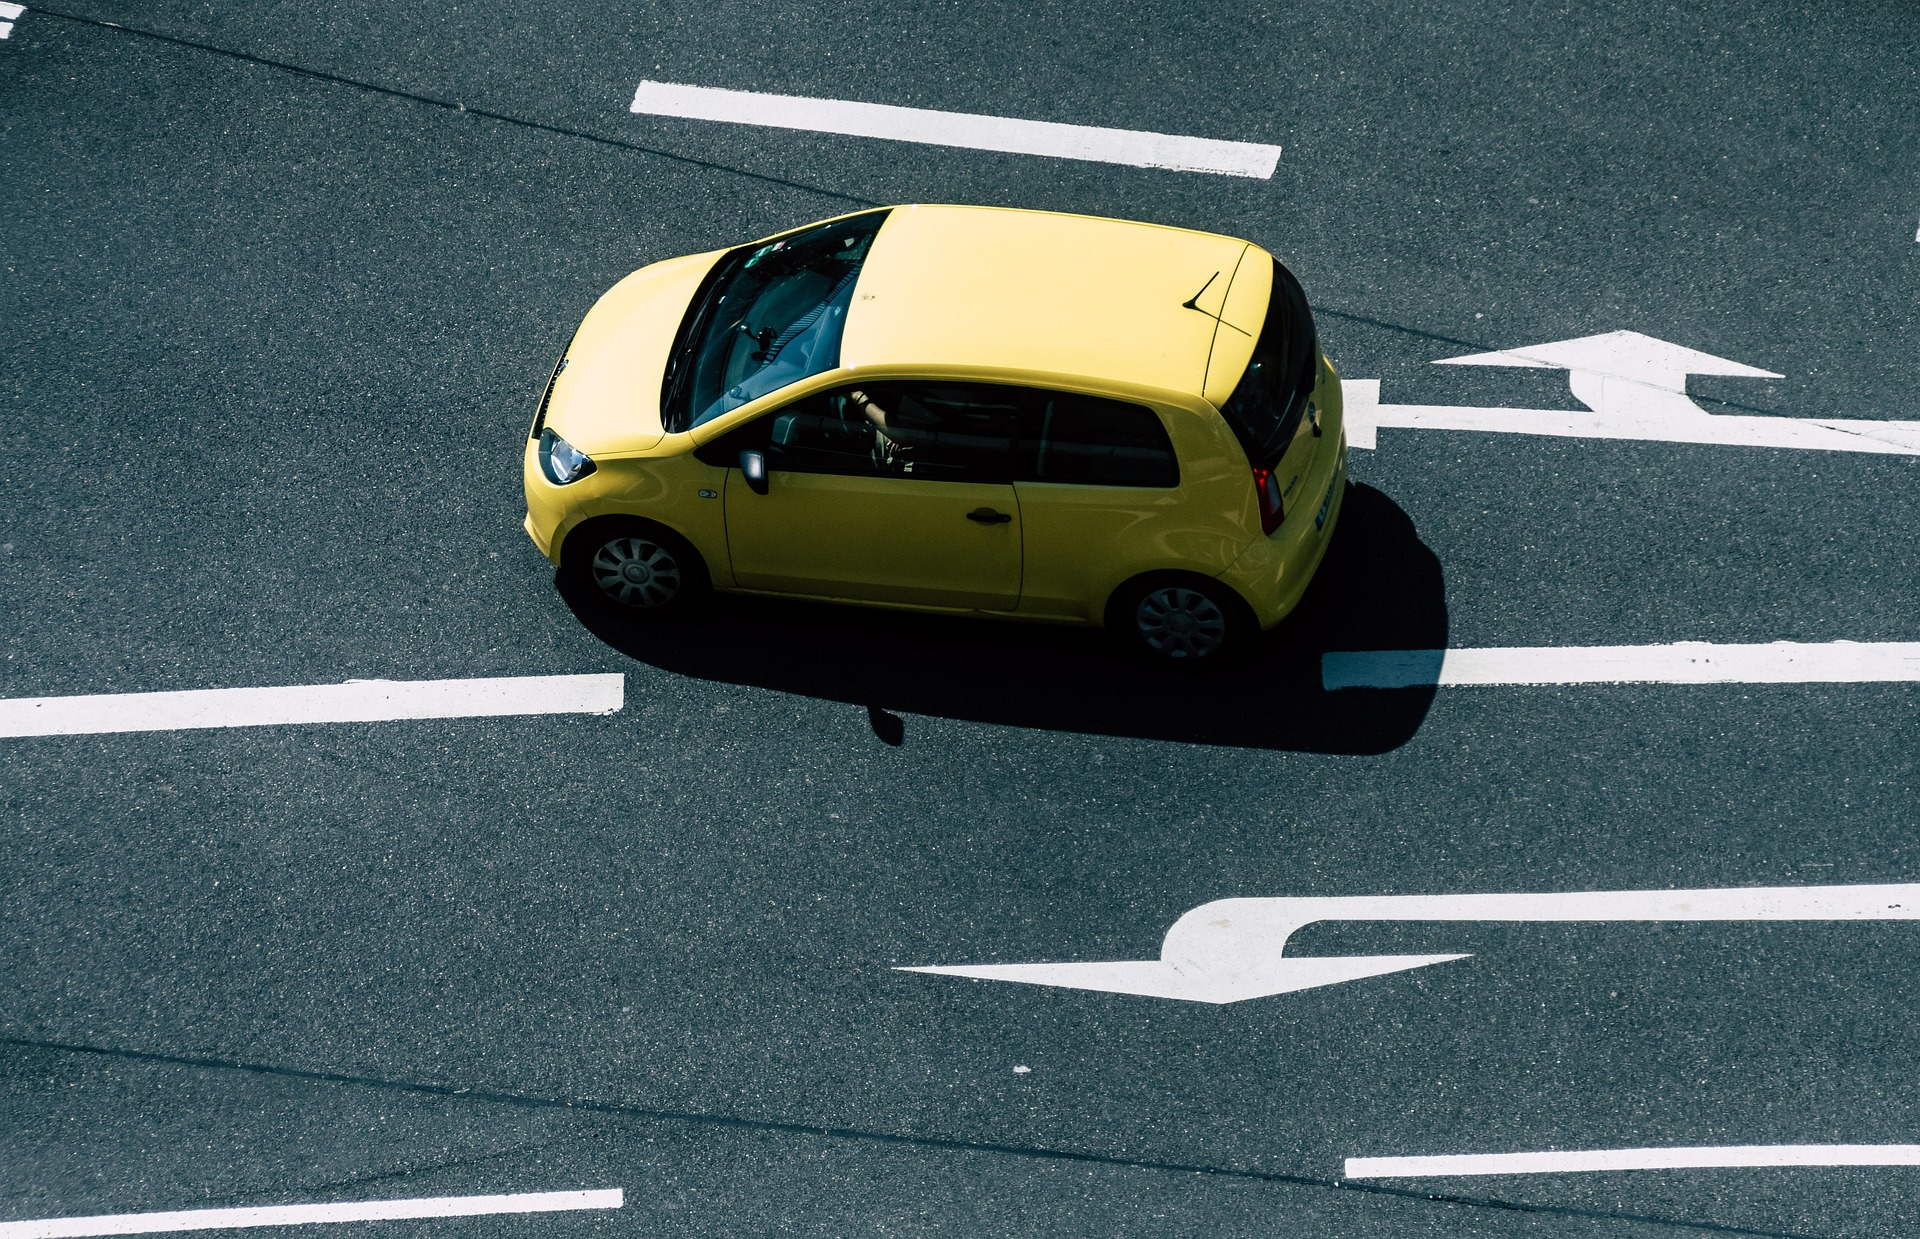
\includegraphics[width=\linewidth,height=0.34\textheight,keepaspectratio]{assets/lane_change_car.jpg}%
      }{%
        \begin{tikzpicture}
          \node[draw,rounded corners,fill=Panel,minimum width=\linewidth,minimum height=0.34\textheight,align=center,text=Muted]
            {lane-change\\image};
        \end{tikzpicture}%
      }
    \end{column}
    \begin{column}{0.48\textwidth}
      \centering
      \begin{tikzpicture}[x=0.82cm,y=0.72cm,>=Latex]
        \draw[->,Muted] (-3.2,0) -- (3.25,0) node[right] {action};
        \draw[->,Muted] (-3.0,0) -- (-3.0,2.4);
        \draw[thick,SignalGreen,domain=-2.8:2.8,samples=100]
          plot (\x,{1.9*exp(-1.8*(\x+1.35)^2) + 1.65*exp(-1.8*(\x-1.35)^2)});
        \draw[dashed,thick,WarmGold] (0,0) -- (0,1.15);
        \node[align=center,font=\scriptsize] at (-1.45,2.1) {merge\\left};
        \node[align=center,font=\scriptsize] at (1.45,2.0) {stay\\straight};
        \node[align=center,text=WarmGold,font=\scriptsize] at (0,-0.42) {mean action};
        \node[draw,rounded corners,fill=Panel,text width=1.25cm,align=center,font=\scriptsize,inner sep=2pt] at (0,1.55) {bad / unsafe};
      \end{tikzpicture}
    \end{column}
  \end{columns}

  \vspace{0.28cm}
  \large
  Consider imitation data for self-driving cars:

  \vspace{0.08cm}
  \normalsize
  \begin{itemize}
    \item in similar observed states, driver 1 stays in lane
    \item driver 2 changes lanes
    \item squared-error regression learns the conditional mean action
  \end{itemize}

  \vspace{0.08cm}
  \textbf{Problem:} the mean action can lie between valid modes: a poor command that no expert demonstrated.
  \note{Use the driving image and action-density plot together. The training set can contain two valid behaviors for similar observed states: staying in lane and changing lanes. Squared-error regression treats these as noisy labels around one target and learns the mean. But the mean action may be a poor steering command that no driver demonstrated. This motivates richer policy distributions such as mixtures, autoregressive policies, or diffusion policies later.}
\end{frame}

\begin{frame}{Pitfall 2: Errors Accumulate Over Time}
  \begin{columns}[T,onlytextwidth]
    \begin{column}{0.48\textwidth}
      \centering
      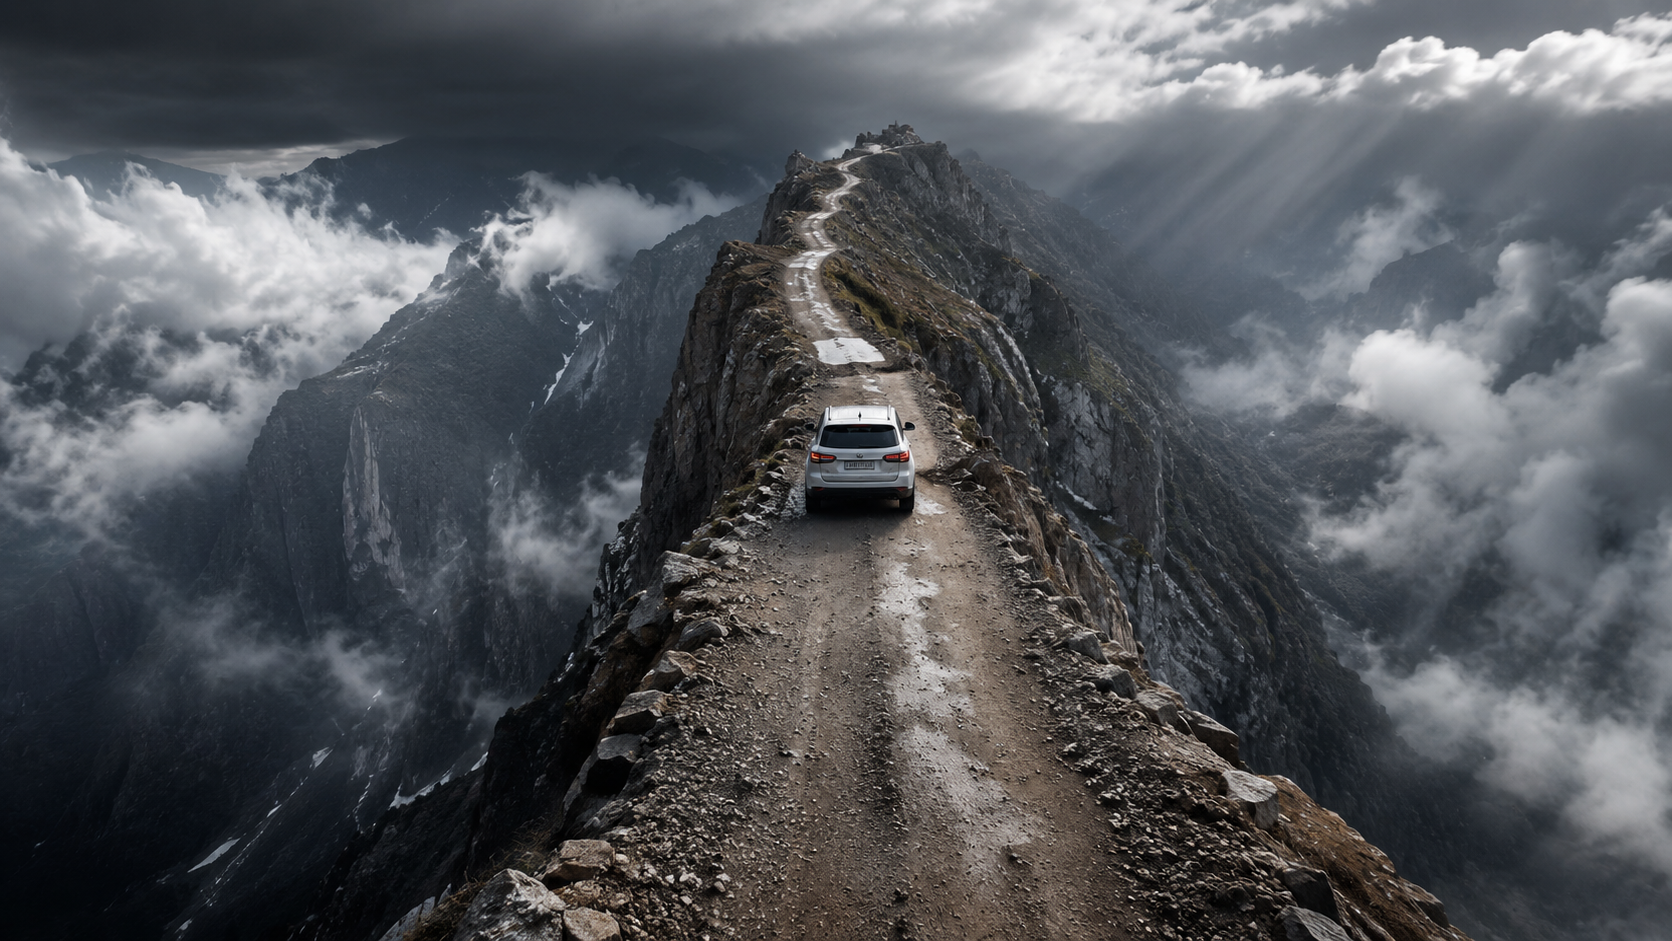
\includegraphics[width=\linewidth,height=0.58\textheight,keepaspectratio]{assets/car-ridge-road.png}
    \end{column}
    \begin{column}{0.48\textwidth}
      \centering
      \begin{tikzpicture}[node distance=0.23cm,>=Latex]
        \tikzset{
          driftstep/.style={
            draw,
            rounded corners,
            fill=Panel,
            text width=0.82\linewidth,
            minimum height=0.78cm,
            align=center
          }
        }
        \node[driftstep] (t0) {$t$: small error};
        \node[driftstep,below=of t0] (t1) {$t{+}1$: shifted state};
        \node[driftstep,below=of t1] (t2) {$t{+}2$: bigger error};
        \node[driftstep,below=of t2] (t3) {$t{+}3$: unfamiliar state};
        \draw[->,thick] (t0) -- (t1);
        \draw[->,thick] (t1) -- (t2);
        \draw[->,thick] (t2) -- (t3);
      \end{tikzpicture}
    \end{column}
  \end{columns}

  \vspace{0.24cm}
  \large
  A policy trained only on expert states may not know how to recover from states caused by its own mistakes.

  \vspace{0.12cm}
  \normalsize
  \begin{itemize}
    \item $\rightarrow$ Distribution shift: deployment samples from the learned policy's state distribution, not the expert's.
  \end{itemize}

  \vspace{0.04cm}
  \textbf{Problem:} one-step prediction errors can look small while long rollouts become unstable.
  \note{Use the ridge-road image to make compounding error visceral. Behavior cloning is trained one step at a time on expert states, but deployment is sequential. If the learned policy is slightly off at time t, the next observation may be shifted away from the expert trajectory. The model is then asked to act on a state it was not trained for, which can create an even larger error at the next step. DAgger is the standard intervention-style fix: collect expert labels on states induced by the learned policy.}
\end{frame}

\begin{frame}{Pitfall 3: Imitation Ignores Outcomes}
  \large
  Behavior cloning asks only:

  \vspace{0.12cm}
  \centering
  \Large
  ``What action was taken in this situation?''

  \vspace{0.28cm}
  \raggedright
  \large
  It does not ask:

  \vspace{0.12cm}
  \centering
  \Large
  ``Which action led to the best long-term outcome?''

  \vspace{0.28cm}
  \raggedright
  \normalsize
  Every logged decision becomes a training example.
  The quality of the outcome does not change how strongly it is learned.

  \vspace{0.14cm}
  \textbf{Problem:} behavior cloning reproduces past decisions, but it cannot prefer decisions with better long-term consequences.
  \note{This is the third limitation of imitation learning. Even if the action distribution is expressive and compounding errors are controlled, behavior cloning still has no signal for which logged choices led to better outcomes. It treats the dataset as behavior to reproduce, not evidence for which actions were valuable. This sets up advantage-weighted regression: keep the supervised-learning structure, but weight demonstrations by how good they were.}
\end{frame}

\begin{frame}{The Offline RL Question}
  \Large
  Given logged grain-terminal decisions and delayed outcomes, can we learn a better policy without risky online experimentation?

  \vspace{0.42cm}
  \normalsize
  Logged data:
  \[
    (s_t, a_t, r_t, s_{t+1})
  \]

  \vspace{0.05cm}
  \begin{itemize}
    \item imitation learning asks: what action was likely in the logs?
    \item offline RL asks: which actions led to better long-term outcomes?
  \end{itemize}

  \vspace{0.12cm}
  This talk focuses on offline RL: policy improvement from fixed data.
  \note{Use this as the transition from behavior cloning to offline RL. Behavior cloning predicts the logged operator action. Offline RL uses logged rewards and next states to ask which actions improved long-term outcomes, while avoiding risky online exploration. This is the main focus of the presentation.}
\end{frame}

\begin{frame}{Rewards: Turning Product Outcomes Into a Learning Signal}
  \Large
  A reward turns delayed product outcomes into feedback for decisions:

  \[
    r_t = r(s_t,a_t,s_{t+1})
  \]

  \vspace{0.25cm}
  \normalsize
  For grain loading, rewards can combine:
  \begin{itemize}
    \item train loading progress and throughput
    \item contract quality satisfaction
    \item penalties for rehandling, congestion, and delay
  \end{itemize}

  \vspace{0.2cm}
  Rewards tell the learner what outcomes matter, not just what actions were taken.
  \note{This slide gives the missing bridge from logged outcomes to RL. A reward is a modeling choice: it translates product objectives and operational costs into a scalar signal that can be optimized over time.}
\end{frame}
